%-------------------------------------------------------------------------------
%	EMPIEZA SECCION
%-------------------------------------------------------------------------------

\section{Motivación}

	Si tomamos como ejemplo el movimiento de un cuerpo en caida libre tendremos que:

	\begin{equation*}
		F = mg = ma = m \frac{d^2 y}{dt^2}
	\end{equation*}

	Si ademas tomamos en cuenta que la masa del cuerpo es unitaria, tenemos que:

	\begin{equation*}
		g = \frac{d^2y}{dt^2} = \frac{dv}{dt}
	\end{equation*}

	por lo que tendremos que la velocidad es:

	\begin{equation*}
		v = \int dv = g \int dt = gt + c
	\end{equation*}

	pero la velocidad tambien puede ser vista como:

	\begin{equation*}
		\frac{dy}{dt} = v = gt + c	
	\end{equation*}

	por lo que:

	\begin{align*}
		y &= \int dy = g \int t dt + \int c dt \\
		y &= \frac{1}{2} gt^2 + ct + d
	\end{align*}

	y por ultimo sabemos las condiciones iniciales del sistema, por lo que podemos saber las constantes involucradas:

	\begin{align*}
		y(0) = 0 &\implies d = 0 \\
		y'(0) = 0 &\implies c = 0
	\end{align*}

	y se reduce a:

	\begin{equation*}
		y = \frac{1}{2} gt^2
	\end{equation*}

	Por otro lado, si consideramos la fricción viscosa del aire tenemos que:

	\begin{align*}
		mg - F_f &= m \frac{d^2 y}{dt^2} \\
		mg - \eta k v &= m \frac{d^2 y}{dt^2} \\
		mg - \bar{k} \frac{dy}{dt} &= m \frac{d^2 y}{dt^2} \quad \bar{k} = \eta k
	\end{align*}

	Se vuelve imposible el simplemente despejar e integrar, por lo que necesitamos una herramienta mas poderosa para resolver este tipo de problemas que aparecen de manera cotidiana en la naturaleza.

%-------------------------------------------------------------------------------
%	EMPIEZA SECCION
%-------------------------------------------------------------------------------

\section{Definiciones}
	
	\begin{definicion}
		Una ecuación diferencial de orden $n$ es una relación de la forma:

		\begin{equation} \label{eq:dif1}
			F(y^{(n)}, y^{(n-1)}, \dots, y', y, x) = 0
		\end{equation}
	\end{definicion}

	\begin{definicion}
		Se dice que $f(a, b) \to \mathbb{R}$ con derivada hasta de orden $n$, es una solución de la ecuación~\ref{eq:dif1} si para todo $x \in (a, b)$, se tiene que:

		\begin{equation}
			F(f^{(n)}(x), f^{(n-1)}(x), \dots, f'(x), f(x), x) = 0
		\end{equation}
	\end{definicion}

	\begin{ejemplo}
		\faltante{Falta escribir ejemplo}
	\end{ejemplo}

	\begin{ejemplo}
		\faltante{Falta escribir ejemplo}
	\end{ejemplo}

	\begin{ejemplo}
		\faltante{Falta escribir ejemplo}
	\end{ejemplo}

	\begin{ejemplo}
		\faltante{Falta escribir ejemplo}
	\end{ejemplo}

	\begin{ejemplo}
		\faltante{Falta escribir ejemplo}
	\end{ejemplo}

	\begin{ejemplo}
		\faltante{Falta escribir ejemplo}
	\end{ejemplo}

	\begin{definicion}
		Para el caso general de una ecuación diferencial tenemos:

		\begin{equation}
			f(x) = a_n y^{(n)} + a_{n-1} y^{(n-1)} + \dots + a_1 y' + a_0 y
		\end{equation}

		La cual podemos ver como un arreglo de variables auxiliares:

		\begin{align}
			x_1 &= y \nonumber\\
			x_2 &= y' \nonumber\\
			& \vdots \nonumber\\
			x_{n-1} &= y^{(n-2)} \nonumber\\
			x_n &= y^{(n-1)}
		\end{align}

		lo cual implica que:

		\begin{align}
			x_1' &= y' = x_2 \nonumber\\
			x_2' &= y'' = x_3 \nonumber\\
			& \vdots \nonumber\\
			x_{n-1}'' &= y^{(n-1)} = x_n \nonumber\\
			x_n' &= y^{(n)}
		\end{align}

		en donde:

		\begin{align*}
			y^{(n)} &= \frac{1}{a_n} \left( f(x) - a_{n-1} y^{n-1} - \dots - a_1 y' - a_0 y \right) \\
			&= \frac{1}{a_n} \left( f(x) - a_{n-1} x_n - \dots - a_1 x_2 - a_0 x_1 \right) \\
			&= \frac{1}{a_n} F(x_1, x_2, \dots, x_n, f(x))
		\end{align*}

		lo cual nos deja a nuestras variables auxiliares como:

		\begin{align}
			x_1' &= y' = x_2 \nonumber\\
			x_2' &= y'' = x_3 \nonumber\\
			& \vdots \nonumber\\
			x_{n-1}'' &= y^{(n-1)} = x_n \nonumber\\
			x_n' &= \frac{1}{a_n} F(x_1, x_2, \dots, x_n, f(x))
		\end{align}

		Si juntamos a todas esta variables en un vector $X$ tenemos que:

		\begin{equation*}
			\dot{X} = A X + f(x)
		\end{equation*}

		o bien, de forma explicita:

		\begin{equation}
			\dot{X} =
			\begin{pmatrix}
				0 & 1 & 0 & \dots & 0 \\
				0 & 0 & 1 & \dots & 0 \\
				0 & 0 & 0 & \dots & 0 \\
				\vdots & \vdots & \vdots & \dots & \vdots \\
				0 & 0 & 0 & \dots & 0 \\
			\end{pmatrix} X +
			\begin{pmatrix}
				0 \\
				0 \\
				0 \\
				\vdots \\
				\frac{1}{a_n} F(x_1, x_2, \dots, x_n, f(x))
			\end{pmatrix}
		\end{equation}

		A esta forma de escribir la ecuación diferencial se le conoce como realización de estado.
	\end{definicion}

%-------------------------------------------------------------------------------
%	EMPIEZA SECCION
%-------------------------------------------------------------------------------
\newpage
\section{Solución de una ecuación diferencial}
	
	\subsection{Ecuaciones diferenciales de primer orden $F(y', y, x) = 0$}

		\begin{definicion}
			La ecuación $F(y', y, x) = 0$ se denomina normal, si se puede despejar la primera derivada, esto es:

			\begin{equation}
				\frac{dy}{dx} = y' = f(x, y)
			\end{equation}
		\end{definicion}

		\begin{definicion}
			La ecuacion $y' = f(x, y)$ se denomina de variables separables, si:

			\begin{equation}
				f(x, y) = \frac{g(x)}{h(y)}
			\end{equation}

			y en este caso la ecuación diferencial se escribe:

			\begin{equation}
				h(y) dy = g(x) dx
			\end{equation}
		\end{definicion}

		\begin{ejemplo}
			La ecuación diferencial:

			\begin{equation*}
				x dx - y dy = 0
			\end{equation*}

			puede ser escrita tambien como:

			\begin{equation*}
				x dx = y dy
			\end{equation*}

			por lo que:

			\begin{equation*}
				\frac{x^2}{2} = \frac{y^2}{2} + c
			\end{equation*}

			y por lo tanto $y$ es de la forma:

			\begin{equation*}
				y = \pm \sqrt{x^2 + c}
			\end{equation*}
		\end{ejemplo}

		\begin{ejemplo}
			Dada la ecuación diferencial:

			\begin{equation*}
				x (1 + y^2) dx - y (1 + x^2) dy = 0
			\end{equation*}

			tenemos que:

			\begin{align*}
				\frac{x (1 + y^2)}{y (1 + x^2)} &= \frac{dy}{dx} \\
				\frac{x}{1 + x^2}dx &= \frac{y}{1 + y^2}dy \\
				\int \frac{x}{1 + x^2}dx &= \int \frac{y}{1 + y^2}dy \\
				\frac{1}{2} \ln{|1 + x^2|} + c &= \frac{1}{2} \ln{|1 + y^2|} \\
				e^{\ln{|1 + x^2|} + c} &= e^{\frac{1}{2} \ln{|1 + y^2|}} \\
				|1 + x^2| e^{\bar{c}} &= |1 + y^2| \\
				|1 + x^2| \tilde{c} &= |1 + y^2|
			\end{align*}
		\end{ejemplo}

		\begin{ejercicio}
			Dada la ecuación diferencial:

			\begin{equation*}
				\frac{dy}{dx} = \cos^2{y} \sin{x}
			\end{equation*}

			Determinar si es de variables separables y resolverla.
		\end{ejercicio}

		\begin{ejercicio}
			Dada la ecuación diferencial:

			\begin{equation*}
				\frac{dy}{dx} + y^2 e^x = y^2
			\end{equation*}

			Determinar si es de variables separables y resolverla.
		\end{ejercicio}

		\begin{definicion}
			Una función $f(x, y)$ se dice homogenea de grado $n$ con $n \in \{0, 1, \dots\}$, si para todo $t > 0$ se tiene que:

			\begin{equation}
				f(tx, ty) = t^n f(x, y)
			\end{equation}
		\end{definicion}

		\begin{ejemplo}
			Dada la función $f(x, y) = x^3 + x y^2$, tenemos que:

			\begin{align*}
				f(tx, ty) &= (tx)^3 + (tx) (ty)^2 \\
				&= t^3 (x^3 + xy^2) \\
				&= t^3 f(x, y)
			\end{align*}

			por lo que $f(x, y)$ es homogenea de grado $3$.
		\end{ejemplo}

		\begin{ejemplo}
			Dada la función $f(x, y) = 1 + \sin{\frac{x}{y}}$, tenemos que:

			\begin{align*}
				f(tx, ty) &= 1 + \sin{\frac{tx}{ty}} \\
				&= 1 + \sin{\frac{x}{y}} \\
				&= t^0 (1 + \sin{\frac{x}{y}}) \\
				&= t^0 f(x, y)
			\end{align*}

			por lo que $f(x, y)$ es homogenea de grado $0$.
		\end{ejemplo}

		\begin{ejemplo}
			Dada la función $f(x, y) = x + \sqrt{x^2 + y^2}$, tenemos que:

			\begin{align*}
				f(tx, ty) &= tx + \sqrt{(tx)^2 + (ty)^2} \\
				&= t (x + \sqrt{x^2 + y^2}) \\
				&= t^1 f(x, y)
			\end{align*}

			por lo que $f(x, y)$ es homogenea de grado $1$.
		\end{ejemplo}

		\begin{definicion}
			Una ecuación $\frac{dy}{dx} = f(x, y)$ se dice homogenea si $f$ es homogenea de grado cero.
		\end{definicion}

		\begin{ejemplo}
			Dada la ecuación $\frac{dy}{dx} = \frac{x + y}{3x - 2y}$, tenemos que:

			\begin{align*}
				f(tx, ty) &= \frac{tx + ty}{3tx - 2ty} \\
				&= \frac{t(x + y)}{t (3x - 2y)} \\
				&= \frac{x + y}{3x - 2y} \\
				&= t^0 f(x, y)
			\end{align*}

			por lo que $f(x, y)$ es homogenea de grado $0$ y por lo tanto esta ecuación es homogenea.
		\end{ejemplo}

		\begin{proposicion}
			Si $M(x, y)$ y $N(x, y)$ son homogeneas del mismo grado $n$, entonces la ecuación diferencial $M(x, y) dx + N(x, y) dy = 0$ es homogenea.
		\end{proposicion}

		\begin{proposicion}
			Si $f(x, y)$ es homogenea de grado cero, entonces podemos establecer la siguiente relacion:

			\begin{equation}
				f(tx, ty) = f(x, y)
			\end{equation}

			Si además $t = \frac{1}{x}$ con $x \ne 0$, tenemos que:

			\begin{equation*}
				f(1, \frac{y}{x}) = f(x, y)
			\end{equation*}

			dadas estas condiciones, tenemos que nuestra ecuación diferencial homogenea queda:

			\begin{equation}
				\frac{dy}{dx} = f(1, \frac{y}{x})
			\end{equation}

			y dado el cambio de variable $z = \frac{y}{x}$, es decir $zx = y$. Esto nos deja con una ecuación diferencial homogenea:

			\begin{equation*}
				\frac{dy}{dx} = \frac{d}{dx}(zx) = x \frac{dz}{dx} + z \frac{dx}{dx} = x \frac{dz}{dx} + z = f(1, z)
			\end{equation*}

			por lo que podemos ver que:

			\begin{equation*}
				\frac{dz}{dx} = \frac{f(1, z) - z}{x}
			\end{equation*}

			y por lo tanto, se puede separar las variables:

			\begin{equation}
				\frac{dz}{f(1, z) - z} = \frac{dx}{x}
			\end{equation}
		\end{proposicion}

		\begin{ejemplo}
			Dada la ecuación $y' = \frac{2x + y}{x}$, podemos ver que con el cambio de variables $z  =\frac{y}{x}$, nos queda:

			\begin{align*}
				x \frac{dz}{dx} + z &= 2 + z \\
				dz &= \frac{2dx}{x} \\
				z = \int dz &= 2 \int \frac{dx}{x} = 2 \ln{x} + c \\
				z &= 2 \ln{x} + c = \frac{y}{x} \\
			\end{align*}

			por lo que la solución de esta ecuación diferencial es:

			\begin{equation*}
				y = 2 x \ln{x} + c x
			\end{equation*}
		\end{ejemplo}

		\begin{ejercicio}
			Dada la ecuación diferencial homogenea $\frac{dy}{dx} = \frac{x + y}{x - y}$, encontrar una solución.
		\end{ejercicio}

		\begin{ejercicio}
			Dada la ecuación diferencial homogenea $\sqrt{x^2 + y^2} dx = y dy$, encontrar una solución.
		\end{ejercicio}

		\begin{definicion}
			Sea $F(x, y)$ tal que:

			\begin{equation}
				dF = \frac{\partial F}{\partial x} dx + \frac{\partial F}{\partial y} dy
			\end{equation}

			Consideremos pues a una ecuación de la forma:

			\begin{equation}
				M(x, y) dx + N(x, y)dy = 0
			\end{equation}

			Ahora, si consideramos a $F$ constante, podemos ver que dado:

			\begin{align*}
				\frac{\partial F}{\partial x} &= M(x, y) \\
				\frac{\partial F}{\partial y} &= N(x, y)
			\end{align*}

			la ecuación diferencial se considerará exacta si existe un $F(x, y)$ tal que:

			\begin{align*}
				M(x, y) &= \frac{\partial F(x, y)}{\partial x} \\
				N(x, y) &= \frac{\partial F(x, y)}{\partial y}
			\end{align*}

			en este caso la ecuación se puede escribir como:

			\begin{equation}
				dF = M(x, y) dx + N(x, y) dy = 0
			\end{equation}
		\end{definicion}

		\begin{ejemplo}
			Dada la ecuación diferencial $y e^x dx + (e^x + 2y) dy = 0$, tenemos que una función $F(x, y)$ de la forma:

			\begin{equation}
			 	F(x, y) = y e^x + y^2 = c
			\end{equation}

			entonces tenemos que:

			\begin{align*}
				\frac{\partial F}{\partial x} &= y e^x \\
				\frac{\partial F}{\partial y} &= e^x + 2y
			\end{align*}
		\end{ejemplo}

		\begin{proposicion}
			Supongase una ecuación:

			\begin{equation}
				M(x, y) dx + N(x, y) dy
			\end{equation}

			esta ecuación es exacta si y solo si:

			\begin{equation}
				\frac{\partial M}{\partial y} = \frac{\partial N}{\partial x}
			\end{equation}
		\end{proposicion}

		Supongase la ecuación $M(x, y) dx + N(x, y) dy$ es exacta, entonces existe un $F(x, y)$ tal que:

			\begin{equation*}
				M = \frac{\partial F}{\partial x}
			\end{equation*}

			y por lo tanto:

			\begin{equation*}
				F = \int M dx + g(y)
			\end{equation*}

			Por otro lado:

			\begin{equation*}
				N = \frac{\partial F}{\partial y}
			\end{equation*}

			y por lo tanto:

			\begin{equation*}
				N = \frac{\partial F}{\partial y} = \frac{\partial}{\partial y} \left[ \int M dx \right] + g'(y)
			\end{equation*}

			por lo que $g(y)$ será de la forma:

			\begin{align*}
				g'(y) &= N - \frac{\partial}{\partial y} \left[ \int M dx \right] \\
				g(y) &= \int \left\{ N - \frac{\partial}{\partial y} \left[ \int M dx \right] \right\} dy
			\end{align*}

			entonces tenemos que $F(x, y)$ queda de la forma:

			\begin{equation*}
				F(x, y) = \int M dx + \int \left\{ N - \frac{\partial}{\partial y} \left[ \int M dx \right] \right\} dy
			\end{equation*}

		\begin{ejemplo}
			Dada la ecuación $y e^x dx + (e^x + 2 y) dy = 0$, por lo que tenemos que:

			\begin{align*}
				M &= y e^x \\
				N &= e^x + 2 y
			\end{align*}

			y al derivar estas ecuaciones tenemos:

			\begin{align*}
				\frac{\partial M}{\partial y} &= e^x \\
				\frac{\partial N}{\partial x} &= e^x
			\end{align*}

			por lo que esta ecuación es exacta, entonces, tenemos que $F(x, y)$ queda:

			\begin{equation*}
				F(x, y) = \int y e^x dx + g(y) = y e^x + g(y)
			\end{equation*}

			si ahora derivamos con respecto a $y$, obtendremos a $N$:

			\begin{equation*}
				\frac{\partial F}{\partial y} = e^x + g'(y) = N = e^x + 2 y
			\end{equation*}

			por lo que:

			\begin{equation*}
				g'(y) = 2 y
			\end{equation*}

			y calculamos $g(y)$:

			\begin{equation*}
				g(y) = \int g'(y) dy = \int 2y dy = y^2 + c
			\end{equation*}

			por lo que $F(x, y)$ queda:

			\begin{equation*}
				F(x, y) = y e^x + y^2 + c
			\end{equation*}
		\end{ejemplo}

		\begin{ejemplo}
			Dada la ecuación $(y + y\cos{(xy)})dx + (x + x\cos{(xy)})dy = 0$ podemos simplificarla de la siguiente manera:

			\begin{align*}
				(y + y\cos{(xy)})dx &+ (x + x\cos{(xy)})dy = 0 \\
				y(1 + \cos{(xy)})dx &+ x(1 + \cos{(xy)})dy = 0 \\
				(y dx + x dy)&(1 + \cos{(xy)}) = 0
			\end{align*}

			Y si asumimos que $1 + \cos{(xy)} \ne 0$, tendremos que $y dx + x dy = 0$, sin embargo asi obtendremos un conjunto reducido de las soluciones de esta ecuación, por lo que procederemos de manera distinta.

			Si asumimos que es de la forma $M dx + N dy = 0$ y derivamos ambas funciones obtendremos:

			\begin{align*}
				\frac{\partial M}{\partial y} &= 1 + \cos{x} \\
				\frac{\partial N}{\partial x} &= 1 + \cos{x} 
			\end{align*}

			por lo que tenemos que es una ecuación exacta y por lo tanto:

			\begin{align*}
				F(x, y) &= \int (y + y \cos{(xy)}) dx + g(y) \\
				&= yx + \sin{(xy)} + g(y)
			\end{align*}

			Si ahora derivamos esto obtendremos $N$:

			\begin{equation*}
				\frac{\partial F}{\partial y} = x + x \cos{(xy)} + g'(y) = x + x \cos{(xy)}
			\end{equation*}

			y por lo tanto:

			\begin{equation*}
				g'(x) = 0
			\end{equation*}

			por lo que si ahora integramos esto, podremos obtener $g(y)$:

			\begin{equation*}
				g(y) = \int g'(y) dy = \int 0 \cdot dy = c
			\end{equation*}

			y por lo tanto, $F(x, y)$ nos queda:

			\begin{equation*}
				F(x, y) = yx + \sin{(xy)} + c
			\end{equation*}
		\end{ejemplo}

		\begin{ejercicio}
			Dada la ecuación $e^x dx + (x e^y + 2y) dy = 0$, investigar si es exacta y obtener su solución.
		\end{ejercicio}

		\begin{ejercicio}
			Dada la ecuación $(2 y^2 - 4 x + 5) dx = (4 - 2 x + 4 x y) dy$, investigar si es exacta y obtener su solución.
		\end{ejercicio}

		\begin{ejercicio}
			Dada la ecuación $(\sin{x} \sin{y} - x e^y) dy = (e^y + \cos{x} \cos{y}) dx$, investigar si es exacta y obtener su solución.
		\end{ejercicio}

%-------------------------------------------------------------------------------
	\newpage
	\subsection{Ecuaciones lineales}

		\begin{definicion}
			Una ecuación diferencial de orden $n$, se dice que es lineal, si es de la forma:

			\begin{equation}
				a_n(x) y^{(n)} + a_{n-1}(x) y^{(n-1)} + \dots + a_1(x) y' + a_0(x) y = f(x)
			\end{equation}
		\end{definicion}

		\begin{definicion}
			Una ecuación diferencial lineal se dice homogenea si $f(x) = 0$ para todo $x$.
		\end{definicion}

		\begin{definicion}
			Una ecuacion diferencial lineal se dice con coeficientes constantes, si $a_n(x), a_{n-1}(x), \dots + a_1(x), a_0(x)$ son funciones constantes.
		\end{definicion}

		\begin{ejemplo}
			La ecuación $2x y'' - x y' = 2$ es una ecuacion lineal de orden dos, con coeficientes variables, no homogenea.
		\end{ejemplo}

		\begin{ejemplo}
			La ecuación $y'' + \lambda^2 y = \cos{(\omega x)}$ es una ecuacion lineal de orden dos, con coeficientes constantes, no homogenea.
		\end{ejemplo}

		Dada una ecuación diferencial lineal, se pueden identificar tres casos para los cuales daremos soluciones con diferentes métodos.

		\begin{enumerate}
			\item Para una ecuación diferencial lineal de la forma:

			\begin{equation}
				a y' + b y = 0
			\end{equation}

			con $a$ y $b$ constantes y $a \ne 0$.

			Dada esta ecuación, podemos ver que:

			\begin{align*}
				a \frac{dy}{dx} &= -b y \\
				\frac{dy}{y} &= -\frac{b}{a} dx \\
				\ln{y} &= -\frac{b}{a} x + c \\
				y &= C e^{-\frac{b}{a} x}
			\end{align*}

			\item Para una ecuación diferencial lineal de la forma:

			\begin{equation}
				a y' + b y = f(x)
			\end{equation}

			con $a$ y $b$ constantes y $a \ne 0$.

			Dada esta ecuación, podemos ver que:

			\begin{align*}
				a y' + b y &= f(x) \\
				y' + \frac{b}{a} y &= \frac{f(x)}{a} \\
				y' + \lambda y &= h(x)
			\end{align*}

			en donde $\lambda = \frac{b}{a}$ y $h(x) = \frac{f(x)}{a}$.
			Por otro lado tenemos que:

			\begin{equation*}
				(e^{\lambda x} y)' = e^{\lambda x} y' + \lambda e^{\lambda x} y = e^{\lambda x} (y' + \lambda y)
			\end{equation*}

			Asi pues, si multiplicamos ambos lados de la ecuación que teniamos por $e^{\lambda x}$, tendremos:

			\begin{align*}
				e^{\lambda x} (y' + \lambda y) &= e^{\lambda x} h(x) \\
				(e^{\lambda x} y)' &= e^{\lambda x} h(x) \\
				e^{\lambda x} y &= \int e^{\lambda x} h(x) dx + c \\
				y &= e^{-\lambda x} \int e^{\lambda x} h(x) dx + e^{-\lambda x}c
			\end{align*}

			\begin{ejemplo}
				Dada la ecuación $y' + 2y = e^{5x}$, tenemos que multiplicando ambos lados por:

				\begin{align*}
					e^{2x}(y' + 2y) &= e^{7x} \\
					(e^{2x} y)' &= e^{7x} \\
					e^{2x} y &= \frac{1}{7} e^{7x} + c \\
					y &= \frac{1}{7} e^{5x} + e^{-2x} c
				\end{align*}
			\end{ejemplo}

			\begin{ejercicio}
				Dada la ecuación $y' + y = x$, obtener el valor de $y$.
			\end{ejercicio}

			\item Para una ecuación lineal de la forma:

			\begin{equation*}
				y' + b(x) y = f(x)
			\end{equation*}

			Podemos proponer una simplificación de la forma:

			\begin{equation*}
				(e^{B(x)} y)' = e^{B(x)}(y' + B'(x) y)
			\end{equation*}

			en donde:

			\begin{equation*}
				B'(x) = b(x)
			\end{equation*}

			por lo que multiplicando ambas partes de la ecuación, por $e^{B(x)}$ se obtiene:

			\begin{align*}
				e^{B(x)}(y' + b(x) y) &= e^{B(x)}f(x) \\
				(e^{B(x)} y)' &= e^{B(x)} f(x) \\
				e^{B(x)} y &= \int e^{B(x)} f(x) dx + c \\
				y &= e^{-B(x)} \int e^{B(x)} f(x) dx + e^{-B(x)}c
			\end{align*}

			\begin{ejemplo}
				Dada la ecuación $y' + \sin{x} y = \sin{x}$, en donde $B(x) = \int \sin{x} dx = - \cos{x}$, por lo que multiplicando ambos lados de la ecuación por $e^{-\cos{x}}$, obtenemos:

				\begin{align*}
					e^{-\cos{x}}(y' + \sin{x} y) &= e^{-\cos{x}} \sin{x} \\
					(e^{-\cos{x}} y)' &= e^{-\cos{x}} \sin{x} \\
					e^{-\cos{x}} y &= \int e^{-\cos{x}} \sin{x} dx \\
					e^{-\cos{x}} y &= e^{-\cos{x}} + c \\
					y &= 1 + Ce^{\cos{x}}
				\end{align*}
			\end{ejemplo}

			\begin{ejercicio}
				Dada la ecuación $y' + xy = x^2$, encontrar el valor de $y$.
			\end{ejercicio}
		\end{enumerate}

%-------------------------------------------------------------------------------
	\newpage
	\subsection{Ecuaciones lineales homogeneas de segundo orden con coeficientes constantes}

		Dada la ecuación:

		\begin{equation}
			y'' + a_1 y' + a_0 y = 0
		\end{equation}

		Supongase que $y = e^{\lambda x}$ es una solución de esta ecuación, por lo que tenemos que: 

		\begin{align*}
			y' &= \lambda e^{\lambda x} \\
			y'' &= \lambda^2 e^{\lambda x}
		\end{align*}

		y sustituyendo en la ecuación tenemos:

		\begin{align*}
			\lambda^2 e^{\lambda x} + a_1 \lambda e^{\lambda x} + a_0 e^{\lambda x} &= 0 \\
			e^{\lambda x} (\lambda^2 + a_1 \lambda + a_0) &= 0
		\end{align*}

		Por lo que para que $e^{\lambda x}$ sea una solución de esta ecuación, $\lambda$ debe cumplir:

		\begin{equation*}
			\lambda^2 + a_1 \lambda + a_0 = 0
		\end{equation*}

		\begin{definicion}
			Al polinomio $P(\lambda) = \lambda^2 + a_1 \lambda + a_0$ se le llama polinomio característico de la ecuación diferencial y a sus raices se les denomina raices caracteristicas.
		\end{definicion}

		\begin{ejemplo}
			Dada la ecuación diferencial:

			\begin{equation*}
				y'' - 3 y' + 2 y = 0
			\end{equation*}

			tenemos que su polinomio caracteristico es:

			\begin{align*}
				\lambda^2 - 3\lambda + 2 &= 0 \\
				(\lambda - 1)(\lambda - 2) &= 0
			\end{align*}

			por lo que sus raices caracteristicas son $\lambda_1 = 1$ y $\lambda_2 = 2$ y por lo tanto:

			\begin{align*}
				y_1 &= e^x \\
				y_2 &= e^{2x}
			\end{align*}

			son soluciones de la ecuación.
		\end{ejemplo}

		\begin{ejemplo}
			Dada la ecuación diferencial:

			\begin{equation*}
				y'' - y = 0
			\end{equation*}

			tenemos que su polinomio caracteristico es:

			\begin{align*}
				\lambda^2 - 1 &= 0 \\
				(\lambda - 1)(\lambda + 1) &= 0
			\end{align*}

			por lo que sus raices caracteristicas son $\lambda_1 = 1$ y $\lambda_2 = -1$ y por lo tanto:

			\begin{align*}
				y_1 &= e^x \\
				y_2 &= e^{-x}
			\end{align*}

			son soluciones de la ecuación.
		\end{ejemplo}

		\begin{teorema}
			Consideremos la ecuación $y'' + a_1 y' + a_0 y = 0$ con $a_1, a_0$ constantes.
			Sean $r_1, r_2$ raices de la ecuación caracteristica $\lambda^2 + a_1 \lambda + a_0 = 0$.
			Si $r_1$ es distinto de $r_2$ definimos:

			\begin{align*}
				\varphi_1(x) &= e^{r_1 x} \\
				\varphi_2(x) &= e^{r_2 x}
			\end{align*}

			Si $r_1 = r_2 = r$ definimos:

			\begin{align*}
				\varphi_1(x) &= e^{rx} \\
				\varphi_2(x) &= x e^{rx}
			\end{align*}

			Entonces, en cualquiera de los casos que definimos, las funciones $\varphi_1, \varphi_2$ son soluciones de la ecuación diferencial.
			Además, cualquier solución $\varphi$ de la ecuación es de la forma:

			\begin{equation}
				y(x) = c_1 \varphi_1(x) + c_2 \varphi_2(x)
			\end{equation}

			con $c_1$ y $c_2$ constantes.
		\end{teorema}

		\begin{proof}
			Supongase que las raices de la ecuación $\lambda^2 + a_1 \lambda + a_0 = 0$ son iguales, es decir, $r_1 = r_2 = r$.
			Sea $\varphi_2(x) = x e^{rx}$, verifiquiemos que $\varphi_2$ es solución de la ecuación.

			\begin{align*}
				\varphi_2'(x) &= (rx + 1) e^{rx} \\
				\varphi_2''(x) &= r(rx + 2) e^{rx}
			\end{align*}

			por lo que sustituyendo en la ecuación diferencial, tenemos:

			\begin{align*}
				r (rx + 2) e^{rx} + a_1 (rx + 1) e^{rx} + a_0 x e^{rx} &= 0 \\
				e^{rx} (r (rx + 2) + a_1 (rx + 1) + a_0 x) &= 0 \\
				e^{rx} (x(r^2 + a_1 r + a_0) + (2r + a_1)) &= 0
			\end{align*}

			y como $r$ es raiz, tenemos que:

			\begin{equation*}
				e^{rx} (2r + a_1) = 0
			\end{equation*}

			y como $r$ es raiz doble tenemos que $r = -\frac{a_1}{2}$, lo cual concuerda con el resultado que obtenemos de aqui:

			\begin{align*}
				2r + a_1 &= 0 \\
				2r &= -a_1 \\
				r &= -\frac{a_1}{2}
			\end{align*}

			Ahora verifiquemos que si $\varphi_1$ y $\varphi_2$ son soluciones de la ecuación, entonces $y = c_1 \varphi_1 + c_2 \varphi_2$ es solución de la ecuación.

			\begin{align*}
				(c_1 \varphi_1'' + c_2 \varphi_2'') + a_1 (c_1 \varphi_1' + c_2 \varphi_2') + a_0 (c_1 \varphi_1 + c_2 \varphi_2) &= 0 \\
				c_1 (\varphi_1'' + a_1 \varphi_1' + a_0 \varphi_1) + c_2 (\varphi_2'' + a_1 \varphi_2' + a_0 \varphi_2) &= 0 \\
				c_1 (0) + c_2 (0) &= 0
			\end{align*}

			por lo tanto, la combinación lineal es solución.
		\end{proof}

		\begin{ejemplo}
			Dada la ecuación $y'' - 4 y' + 4 y = 0$ su polinomio caracteristico es:

			\begin{align*}
				\lambda^2 - 4 \lambda + 4 &= 0 \\
				(\lambda - 2)^2 &= 0
			\end{align*}

			por lo que las raices caracteristicas $\lambda_1 = \lambda_2 = 2$, y por lo tanto las soluciones para esta ecuación son:

			\begin{align*}
				\varphi_1(x) &= x e^{2x} \\
				\varphi_2(x) &= e^{2x}
			\end{align*}

			mas aun, la solución general es $\varphi(x) = c_1 x e^{2x} + c_2 e^{2x}$.
		\end{ejemplo}

		\begin{ejercicio}
			Dada la ecuación $y'' - 4 y' + 5 y = 0$, encontrar la solución general.
		\end{ejercicio}

		\begin{ejercicio}
			Dada la ecuación $y'' + 2 y' + y = 0$, encontrar la solución general.
		\end{ejercicio}

		\begin{ejercicio}
			Dada la ecuación $y'' + 8 y = 0$, encontrar la solución general.
		\end{ejercicio}

		\begin{ejercicio}
			Dada la ecuación $y'' - 9 y' + 20 y = 0$, encontrar la solución general.
		\end{ejercicio}

		\begin{ejercicio}
			Dada la ecuación $2 y'' + 2 y' + 3 y = 0$, encontrar la solución general.
		\end{ejercicio}

		\begin{ejercicio}
			Verifique que la derivada de cualquier solución de la ecuación:

			\begin{equation*}
				y'' + a_1 y' + a_0 y = 0
			\end{equation*}

			es tambien una solución de esta.
		\end{ejercicio}

%-------------------------------------------------------------------------------
	\newpage
	\subsection{Ecuaciones lineales no homogeneas de segundo orden con coeficientes constantes}

		\begin{definicion}
			Sea la ecuación:

			\begin{equation} \label{eq:lin1}
				y'' + a_1 y' + a_0 y = b(x)
			\end{equation}

			una ecuación diferencial lineal no homogenea de segundo orden con coeficientes constantes.
		\end{definicion}

		\begin{teorema}
			Si $\varphi_1$ y $\varphi_2$ son soluciones de la ecuación~\ref{eq:lin1}, $\varphi_p$ es cualquier solución de la ecuación~\ref{eq:lin1}, es decir, es solución particular de la ecuación\ref{eq:lin1}.

			Entonces la solución general esta dada por:

			\begin{equation}
				\varphi(x) = c_1 \varphi_1(x) + c_2 \varphi_2(x) + \varphi_p(x)
			\end{equation}
		\end{teorema}

		Se reemplazan las constantes $c_1$ y $c_2$ por funciones $\mu_1(x)$ y $\mu_2(x)$ y se trata de determinar $\mu_1$ y $\mu_2$ de tal modo que $y = \mu_1 \varphi_1 + \mu_2 \varphi_2$ es una solución de la ecuación.

		El objetivo es hallar $\mu_1$ y $\mu_2$ tales que $\mu_1 \varphi_1 + \mu_2 \varphi_2$ es solución de la ecuación no homogenea.

		Sea $y = \mu_1 \varphi_1 + \mu_2 \varphi_2$, entonces:

		\begin{align*}
			y' &= \mu_1 \varphi_1' + \mu_1' \varphi_1 + \mu_2 \varphi_2' + \mu_2' \varphi_2 \\
			y'' &= \mu_1 \varphi_1'' + \mu_1' \varphi_1' + \mu_1' \varphi_1' + \mu_1'' \varphi_1 + \mu_2 \varphi_2'' + \mu_2' \varphi_2' + \mu_2' \varphi_2' + \mu_2'' \varphi_2
		\end{align*}

		y sustituyendo en la ecuación, tenemos:

		\begin{multline*}
			\mu_1 \varphi_1'' + \mu_1' \varphi_1' + \mu_1' \varphi_1' + \mu_1'' \varphi_1 + \mu_2 \varphi_2'' + \mu_2' \varphi_2' + \mu_2' \varphi_2' + \mu_2'' \varphi_2 \\
			+ a_1 \mu_1 \varphi_1' + a_1 \mu_1' \varphi_1 + a_1 \mu_2 \varphi_2' + a_1 \mu_2' \varphi_2 \\
			+ a_0 \mu_1 \varphi_1 + a_0 \mu_2 \varphi_2 = b(x)
		\end{multline*}

		y recolectando los terminos con respecto a los $\mu$, tenemos que:

		\begin{multline*}
			\mu_1 (\varphi_1'' + a_1 \varphi_1' + a_0 \varphi_1) + \mu_2 (\varphi_2'' + a_1 \varphi_2' + a_0 \varphi_2) \\
			+ \mu_1' \varphi_1' + \mu_1' \varphi_1' + \mu_1'' \varphi_1 + \mu_2' \varphi_2' + \mu_2' \varphi_2' + \mu_2'' \varphi_2 \\
			+ a_1 \mu_1' \varphi_1 + a_1 \mu_2' \varphi_2 = b(x)
		\end{multline*}

		y ya que $\varphi_1$ y $\varphi_2$ son soluciones del sistema, esta ecuación se reduce a:

		\begin{multline*}
			\mu_1' \varphi_1' + \mu_1' \varphi_1' + \mu_1'' \varphi_1 + \mu_2' \varphi_2' + \mu_2' \varphi_2' + \mu_2'' \varphi_2 \\
			+ a_1 \mu_1' \varphi_1 + a_1 \mu_2' \varphi_2 = b(x)
		\end{multline*}

		Por otro lado, notamos que:

		\begin{equation*}
			(\mu_1' \varphi_1 + \mu_2' \varphi_2)' = \mu_1' \varphi_1' + \mu_1'' \varphi_1 + mu_2' \varphi_2' + \mu_2'' \varphi_2
		\end{equation*}

		por lo que podemos plantear una realización de estado:

		\begin{align*}
			\mu_1' \varphi_1 + \mu_2' \varphi_2 &= 0 \\
			\mu_1' \varphi_1' + \mu_1'' \varphi_1 + mu_2' \varphi_2' + \mu_2'' \varphi_2 &= b(x)
		\end{align*}

		para resolver con respecto a $\mu_1'$ y $\mu_2'$ por lo que podemos plantear que obteniendo el Wronskiano, podemos saber si el sistema tiene solución.

		\begin{equation}
			W(\varphi_1, \varphi_2) =
			\begin{vmatrix}
				\varphi_1 & \varphi_2 \\
				\varphi_1' & \varphi_2'
			\end{vmatrix} = \varphi_1 \varphi_2' - \varphi_2 \varphi_1' \ne 0
		\end{equation}

		teniendo este Wronskiano, o determinante del sistema, podemos obtener $\mu_1$ y $\mu_2$:

		\begin{align*}
			\mu_1' &= \frac{\begin{vmatrix} 0 & \varphi_2 \\ b(x) & \varphi_2' \end{vmatrix}}{W(\varphi_1, \varphi_2)} = -\frac{b(x) \varphi_2}{W(\varphi_1, \varphi_2)} \\
			\mu_2' &= \frac{\begin{vmatrix} \varphi_1 & 0 \\ \varphi_1' & b(x) \end{vmatrix}}{W(\varphi_1, \varphi_2)} = \frac{b(x) \varphi_1}{W(\varphi_1, \varphi_2)}
		\end{align*}

		y por lo tanto:

		\begin{align*}
			\mu_1 &= - \int \frac{b(x) \varphi_2}{W(\varphi_1, \varphi_2)} dx \\
			\mu_2 &= \int \frac{b(x) \varphi_1}{W(\varphi_1, \varphi_2)} dx
		\end{align*}

		\begin{ejemplo}
			Dada la ecuación $y'' - 2 y' + y = 2x$ su polinomio caracteristico es $\lambda^2 - 2 \lambda + 1 = 0$, por lo que tenemos que las raices caracteristicas son $\lambda_1 = \lambda_2 = 1$ y las soluciones $\varphi_1$ y $\varphi_2$ son:

			\begin{align*}
				\varphi_1 &= e^x \\
				\varphi_2 &= x e^x
			\end{align*}

			y derivando ambas soluciones tenemos:

			\begin{align*}
				\varphi_1' &= e^x \\
				\varphi_2' &= (1 + x) e^x
			\end{align*}

			Calculando el determinante del sistema, tenemos:

			\begin{equation*}
				W(\varphi_1, \varphi_2) = (1 + x) e^x e^x - x e^x e^x = e^{2x} \ne 0
			\end{equation*}

			y tenemos que las $\mu$ son:

			\begin{align*}
				\mu_1 &= - \int \frac{x e^x 2x}{e^{2x}} dx = 2 e^{-x} (x^2 + 2 x + 2) \\
				\mu_2 &= \int \frac{e^x 2x}{e^{2x}} dx = -2 e^{-x}(x + 1)
			\end{align*}

			y sustituyendo en la forma de la solución general $y = \mu_1 \varphi_1 + \mu_2 \varphi_2$, tenemos:

			\begin{align*}
				y &= (2 e^{-x} (x^2 + 2 x + 2)) e^x + (-2 e^{-x}(x + 1)) x e^x \\
				&= (2 x^2 + 4 x + 4) + (-2 x^2 - 2 x) \\
				&= 2 (x + 2)
			\end{align*}
		\end{ejemplo}

		\begin{ejemplo}
			Dada la ecuación $y'' - y' - 6 y = e^{-x}$ su polinomio caracteristico  es $\lambda^2 - \lambda - 6 = 0$, por lo que tenemos que las raices caracteristicas son $\lambda_1 = 3$ y $\lambda_2 = -2$ y las soluciones $\varphi_1$ y $\varphi_2$ son:

			\begin{align*}
				\varphi_1 &= e^{3x} \\
				\varphi_2 &= e^{-2x}
			\end{align*}

			y derivando ambas soluciones tenemos:

			\begin{align*}
				\varphi_1' &= 3e^{3x} \\
				\varphi_2' &= -2e^{-2x}
			\end{align*}

			Calculando el determinante del sistema, tenemos:

			\begin{equation*}
				W(\varphi_1, \varphi_2) = -2 e^{3x} e^{-2x} - 3 e^{3x} e^{-2x} = -5 e^{x} \ne 0
			\end{equation*}

			y tenemos que las $\mu$ son:

			\begin{align*}
				\mu_1 &= - \int \frac{e^{-x} e^{-2x}}{-5 e^{x}} dx = - \frac{1}{20} e^{-4x} \\
				\mu_2 &= \int \frac{e^{-x} e^{3x}}{-5 e^{x}} dx = - \frac{1}{5} e^x
			\end{align*}

			y sustituyendo en la forma de la solución general $y = \mu_1 \varphi_1 + \mu_2 \varphi_2$, tenemos:

			\begin{align*}
				y &= (- \frac{1}{20} e^{-4x}) e^{3x} + (- \frac{1}{5} e^x) e^{-2x} \\
				&= -\frac{1}{20} e^{-x} - \frac{1}{5} e^{-x} \\
				&= -\frac{1}{4} e^{-x}
			\end{align*}
		\end{ejemplo}

		\begin{ejercicio}
			Dada la ecuación $y'' + 4 y = \tan{2x}$, obtener la solución general a la ecuación.
		\end{ejercicio}

		\begin{ejercicio}
			Dada la ecuación $y'' + 2 y' + y = e^{-x} \ln{x}$, obtener la solución general a la ecuación.
		\end{ejercicio}

		\begin{ejercicio}
			Dada la ecuación $y'' - 2 y' - 3 y = x e^{-x}$, obtener la solución general a la ecuación.
		\end{ejercicio}

		\begin{ejercicio}
			Dada la ecuación $y'' + 2 y' + 5 y = e^{-x} \sec{2x}$, obtener la solución general a la ecuación.
		\end{ejercicio}

%-------------------------------------------------------------------------------
%	EMPIEZA SECCION
%-------------------------------------------------------------------------------
\newpage
\section{Existencia y unicidad de las soluciones de una ecuación diferencial}

	\subsection{Problemas con condiciones iniciales}

		\begin{teorema}
			Dados $x_0, \alpha, \beta \in \mathbb{R}$, existen las constantes únicas $c_1$ y $c_2$, tales que la función:

			\begin{equation}
				\varphi(x) = c_1 \varphi_1 + c_2 \varphi_2
			\end{equation}

			satisfacen $\varphi(x_0) = \alpha$ y $\varphi'(x_0) = \beta$ y las funciones $\varphi_1$ y $\varphi_2$ estan dadas por:

			\begin{enumerate}
				\item $\varphi_1(x) = e^{r_1 x}$ y $\varphi_2(x) = e^{r_2 x}$ para $r_1 \ne r_2$.
				\item $\varphi_1(x) = e^{rx}$ y $\varphi_2(x) = x e^{rx}$ para $r_1 = r_2 = r$.
			\end{enumerate}
		\end{teorema}

		\begin{proof}
			Se requiere que $c_1$ y $c_2$ sean tales que:

			\begin{align*}
				c_1 \varphi_1(x_0) + c_2 \varphi_2(x_0) = \alpha &= \varphi(x_0) \\
				c_1 \varphi_1'(x_0) + c_2 \varphi_2'(x_0) = \beta &= \varphi(x_0)
			\end{align*}

			Este sistema tiene solución, pues su determinante es diferente de cero en cualquiera de los dos casos.
			En efecto:

			\begin{equation*}
				A =
				\begin{vmatrix}
					\varphi_1(x_0) & \varphi_2(x_0) \\
					\varphi_1'(x_0) & \varphi_2'(x_0)
				\end{vmatrix} = \varphi_1(x_0) \varphi_2'(x_0) - \varphi_2(x_0) \varphi_1'(x_0)
			\end{equation*}

			Consideremos ahora cada uno de los casos.
			Para el caso en que $r_1 \ne r_2$ tenemos que:

			\begin{equation*}
				W(\varphi_1, \varphi_2) =
				\begin{vmatrix}
					e^{r_1 x} & e^{r_2 x} \\
					r_1 e^{r_1 x} & r_2 e^{r_2 x}
				\end{vmatrix} = (r_2 - r_1) e^{(r_1 + r_2) x} \ne 0
			\end{equation*}

			Y para el caso en que $r_1 = r_2 = r$:

			\begin{equation*}
				W(\varphi_1, \varphi_2) =
				\begin{vmatrix}
					e^{r x} & x e^{r x} \\
					r e^{r x} & (1 + x) e^{r x}
				\end{vmatrix} = e^{2 r x} \ne 0
			\end{equation*}

			De aqui, que la solución es única para $c_1$ y $c_2$ en:

			\begin{equation*}
				\varphi = c_1 \varphi_1 + c_2 \varphi_2
			\end{equation*}
		\end{proof}

		\begin{proposicion}
			Si $\varphi_1$ y $\varphi_2$ son soluciones de la ecuación $y'' + a_1 y' + a_0 y = 0$, entonces existe $A$, tal que:

			\begin{equation}
				W(\varphi_1, \varphi_2) = A e^{-a_1 x}
			\end{equation}
		\end{proposicion}

		\begin{proof}
			Por hipotesis, tenemos que:

			\begin{align*}
				\varphi_1'' + a_1 \varphi_1' + a_0 \varphi_1 &= 0 \\
				\varphi_2'' + a_1 \varphi_2' + a_0 \varphi_2 &= 0
			\end{align*}

			Si a la primer ecuación la multiplicamos por $\varphi_2$ y la primera por $\varphi_1$, la resta de estas dos nos dará:

			\begin{equation*}
				(\varphi_1 \varphi_2'' - \varphi_2 \varphi_1'') + a_1 (\varphi_1 \varphi_2' - \varphi_2 \varphi_1') = 0
			\end{equation*}

			Por otro lado, el Wronskiano nos da:

			\begin{equation*}
				W(\varphi_1, \varphi_2) =
				\begin{vmatrix}
					\varphi_1 & \varphi_2 \\
					\varphi_1' & \varphi_2'
				\end{vmatrix} = \varphi_1 \varphi_2' - \varphi_2 \varphi_1'
			\end{equation*}

			y este tiene una derivada de la forma:

			\begin{align*}
				\frac{d W}{dx} &= (\varphi_1 \varphi_2'' + \varphi_2' \varphi_1') - (\varphi_2 \varphi_1'' + \varphi_2' \varphi_1') \\
				&= \varphi_1 \varphi_2'' - \varphi_2 \varphi_1''
			\end{align*}

			por lo que tenemos que:

			\begin{equation*}
				\frac{dW}{dx} + a_1 W = 0
			\end{equation*}

			lo cual escrito de manera diferente es:

			\begin{align*}
				\frac{dW}{W} &= - a_1 dx \\
				\ln{W} &= -a_1 x + c \\
				W &= e^{-a_1 x + c} \\
				W &= A e^{-a_1 x}
			\end{align*}

			en donde $A = e^{c}$
		\end{proof}

		\begin{observacion}
			Considerese la ecuación $y'' + a_1 y' + a_0 y = 0$, si la raices caracteristicas son complejas, es decir $r_1 = a + b i$ y $r_2 = a - b i$, con $b \ne 0$, entonces la solución general de la ecuación diferencial se pueden simplificar a la forma:

			\begin{equation*}
				\varphi(x) = A e^{a x} \cos{(b x)} + B e^{a x} \sin{(b x)}
			\end{equation*}
		\end{observacion}

		\begin{proof}
			Podemos sustituir las soluciones complejas generales en la solución general para esta ecuación y verificar que:

			\begin{align*}
				\varphi(x) &= c_1 e^{r_1 x} + c_2 e^{r_2 x} \\
				\varphi(x) &= c_1 e^{(a + b i) x} + c_2 e^{(a - b i) x} \\
				\varphi(x) &= c_1 e^{a x} e^{bi x} + c_2 e^{a x} e^{-bi x} \\
				\varphi(x) &= e^{ax} (c_1 e^{bi x} + c_2 e^{-bi x}) \\
				\varphi(x) &= e^{ax} \left[ c_1 (\cos{(bx)} + i \sin{(bx)}) + c_2 (\cos{(bx)} - i \sin{(bx)}) \right] \\
				\varphi(x) &= e^{ax} \left[ (c_1 + c_2) \cos{(bx)} + (c_1 - c_2) i \sin{(bx)} \right] \\
			\end{align*}

			Si definimos ahora $A = c_1 + c_2$ y $B = i(c_1 - c_2)$ podremos escribir a $\varphi(x)$ como:

			\begin{equation*}
				\varphi(x) = A e^{ax} \cos{(b x)} + B e^{a x} \sin{(b x)}
			\end{equation*}

			En particular, tenemos las siguientes soluciones:

			\begin{align*}
				\varphi_1(x) &= e^{ax} \cos{(b x)} \\
				\varphi_2(x) &= e^{ax} \sin{(b x)}
			\end{align*}

			Por lo que el determinante del sistema queda:

			\begin{equation*}
				W(\varphi_1, \varphi_2) =
				\begin{vmatrix}
					e^{a x} \cos{(b x)} & e^{a x} \sin{(b x)} \\
					e^{a x} (a\cos{(b x)} - b \sin{(b x)}) & e^{a x} ((a\sin{(b x)} - b \cos{(b x)}))
				\end{vmatrix} = b e^{2 a x} \ne 0
			\end{equation*}

			Por lo que el sistema tiene soluciones únicas.
		\end{proof}

		\begin{ejemplo}
			\faltante{Falta escribir ejemplo}
		\end{ejemplo}

		\begin{ejercicio}
			Verificar que la ecuación diferencial:

			\begin{equation*}
				y' + P(x) y = Q(x) y^n
			\end{equation*}

			puede ser reducida a una ecuación diferencial lineal mediante la sustitución:

			\begin{equation*}
				z = y^{-(n-1)}
			\end{equation*}

			y dar la solución general.
		\end{ejercicio}

%-------------------------------------------------------------------------------
	\newpage
	\subsection{Soluciones particulares de ecuaciones lineales de segundo orden con coeficientes constantes}

		\begin{ejemplo}
			Dada la ecuación $y'' + 2 y' + y = 5$, tenemos que $y = 5$ es una solución particular.
		\end{ejemplo}

		\begin{ejemplo}
			Dada la ecuación $y'' + y' - y = 3x$, tenemos que $y = -3x - 3$ es una solución particular.
		\end{ejemplo}

		\begin{ejemplo}
			Dada la ecuación $y'' + 5 y' + 2 y = 2 x$, econtremos una solución particular, proponiendo una solucion de la forma $\varphi(x) = a x + b$, con lo que $\varphi'(x) = a$ y $\varphi''(x) = 0$, sustituyendo tenemos:

			\begin{equation*}
				0 + 5 (a) + 2 (a x + b) = 2 x
			\end{equation*}

			por lo que tenemos el sistema:

			\begin{align*}
				2a &= 2 \\
				5a + 2b &= 0
			\end{align*}

			por lo que tenemos que $a = 1$ y $b = - \frac{5}{2}$, es decir la solución particular es:

			\begin{equation*}
				\varphi(x) = x - \frac{5}{2}
			\end{equation*}
		\end{ejemplo}

		\begin{ejercicio}
			Dada la ecuación $y'' + 6 y = 2 x^2 + x - 3$, encontrar la solución particular de esta ecuación.
		\end{ejercicio}

		\begin{ejercicio}
			Dada la ecuación $y'' + 2 y' + y = \sin{x}$, encontrar la solución particular de esta ecuación.
		\end{ejercicio}

		\begin{observacion}
			Supongamos la ecuación:

			\begin{equation}
				y'' + a_1 y' + a_0 y = b(x)
			\end{equation}

			Para obtener la solución particular de una ecuación debemos determinar el tipo de función que utilizaremos como propuesta de solución.

			\begin{enumerate}
				\item Si $b(x) = a_n x^n + \dots + a_1 x + a_0$ se propone un polinomio del mismo grado y se determinan los coeficientes $\alpha_i$, entonces:

				\begin{equation*}
					\varphi_p = \alpha_n x^n + \dots + \alpha_1 x + \alpha_0
				\end{equation*}

				\item Si $b(x) = A \sin{(\omega x)} + B \cos{(\omega x)}$ se propone una solución:

				\begin{equation*}
					\varphi_p = \alpha \sin{(\omega x)} + \beta \cos{\omega x}
				\end{equation*}

				aun si $A$ o $B$ son cero.

				\item Si $b(x) = a e^{kx}$, se propone un $\varphi_p = A e^{kx}$ y se tiene que:
				
				\begin{align*}
					\varphi_p(x) &= A e^{kx} \\
					\varphi_p'(x) &= Ak e^{kx} \\
					\varphi_p''(x) &= Ak^2 e^{kx} \\
				\end{align*}

				y por lo tanto, al sustituir en la ecuación original, tenemos que:

				\begin{align*}
					A (k^2 + a_1 k + a_0) e^{kx} &= a e^{kx} \\
					A &= \frac{a}{(k^2 + a_1 k + a_0)}
				\end{align*}
			\end{enumerate}
		\end{observacion}

		\begin{observacion}
			Considerese la ecuación:

			\begin{equation}
				y'' + a_1 y' + a_0 y = b(x)
			\end{equation}

			Para aplicar el método, $b(x)$ debe satisfacer lo siguiente:

			Existen $b_1, b_2, \dots, b_n$ tal que cualquiers derivada $b^{(k)}(x)$ debe poderse escribir como combinación lineal de ellas, la manera de darse cuenta de este hecho, es derivando $b(x)$ un número suficientemente grande de veces y observando que despues de un cierto orden de la derivada todos los terminos que aparecen son repetidos.
		\end{observacion}

%-------------------------------------------------------------------------------
%	EMPIEZA SECCION
%-------------------------------------------------------------------------------
\newpage
\section{Soluciones aproximadas}

	\subsection{Series de potencias}

		\begin{definicion}
			Dada una sucesión $(a_n)_{n=1}^{\infty}$ la serie termino general $a_n$ es la sucesión $(s_n)_{n=1}^{\infty}$ definida por:

			\begin{align*}
				s_1 &= a_1 \\
				s_2 &= a_1 + a_2 \\
				s_n &= a_1 + a_2 + \dots + a_n \\
				(s_n) &= \sum_{k=1}^n a_k \\
				(s_n)_{n=1}^{\infty} &= \left( \sum_{k=1}^{n} a_k \right)_{n=1}^{\infty}
			\end{align*}

			Esta sucesión tambien será denotada por $\sum a_n$.
			Si el indice de los $a_n$ comienza desde $n_0$, es decir se tiene la sucesion $(a_n)_{n=n_0}^{\infty}$, escribimos $\sum_{n=n_0} a_n$ en lugar de $\sum a_n$.

			A los terminos de la serie $\sum a_n$ ($s_1, s_2, \dots$) se les llama sumas parciales de la serie y se dice que $\sum a_n$ converge si la sucesión $a_1, a_1 + a_2,  a_1 + a_2 + \dots + a_n$ converge.
		\end{definicion}

%-------------------------------------------------------------------------------
	\newpage
	\subsection{Criterio de Cauchy}

		Si una serie converge, denotaremos a su limite por:

		\begin{equation}
			\sum_{n=1}^{\infty} a_n
		\end{equation}

		o mas generalmente:

		\begin{equation}
			\sum_{n=n_0}^{\infty} a_n
		\end{equation}

		$(s_n)$ converge si y solo si para cada $\epsilon > 0$ existe un $n_0$ tal que $n, m < n_0$ implica que:

		\begin{equation}
			|s_n - s_m| < \epsilon
		\end{equation}

		Otra formulación para el criterio de Cauchy es la siguiente:

		Una suceción $(s_n)$ converge si y solamente si existe un $n_0$ tal que $n \geq n_0$ y $p \geq 1$ tales que:

		\begin{equation*}
			|s_{n+p} - s_n| \leq \epsilon
		\end{equation*}

		es decir:

		\begin{equation*}
			\left( \sum_{k=1}^{n+p} a_k - \sum_{k=1}^{n} a_k \right) = \sum_{k=n+1}^{n+p} a_k = \sum_{k=1}^{p} a_{n+k} \leq \epsilon
		\end{equation*}

		Una serie $\sum a_n$ converge si y solamente si para cada $\epsilon > 0$, existe un $n_0$ tal que $n \geq n_0$, $p \geq 1$, tales que:

		\begin{equation}
			\left| \sum_{k=1}^{p} a_{n+k} \right| < \epsilon
		\end{equation}

%-------------------------------------------------------------------------------
	\newpage
	\subsection{Criterio de la razon para la convergencia de una serie}

		\begin{teorema}
			Suponga una serie $\sum a_n$ con $a_n \ne 0$ para toda $n$ tal que existe el limite:

			\begin{equation}
				\lim_{n \to \infty} \frac{a_{n+1}}{a_n} = \alpha
			\end{equation}

			Podemos ver los siguientes casos:

			\begin{enumerate}
				\item Si $\alpha < 1$ la serie converge.
				\item Si $\alpha > 1$ la serie diverge.
				\item Si $\alpha = 1$ no se puede decir nada acerca de la serie.
			\end{enumerate}
		\end{teorema}

		\begin{ejemplo}
			\faltante{Falta escribir ejemplo}
		\end{ejemplo}

		\begin{ejemplo}
			\faltante{Falta escribir ejemplo}
		\end{ejemplo}

		\begin{definicion}
			Sea $a_n$ una sucesión y $x_0 \in \mathbb{R}$ para cada $x \in \mathbb{R}$ definamos la serie $\sum a_n (x - x_0)^n$.
		\end{definicion}

		\begin{teorema}
			Considerese la serie de potencias $\sum a_n(x - x_0)^n$, entonces existe $R$, con $0 \leq R \leq \infty$ tal que la serie $\sum a_n (x - x_0)^n$.

			Entonces se puede decir lo siguiente de esta serie:

			\begin{enumerate}
				\item Converge si $|x - x_0| < R$.
				\item Diverge si $|x - x_0| > R$.
			\end{enumerate}

			Por otro lado podemos decir lo siguiente con respecto $R$:

			\begin{enumerate}
				\item Si $R = 0$ la serie converge solamente en $x = x_0$.
				\item Si $R = \infty$ la serie converge para todo $x$.
			\end{enumerate}

			Si ahora utilizamos el teorema de Cauchy, podemos ver que:

			\begin{align*}
				\alpha &= \lim_{n \to \infty} \left| \frac{a_{n+1}(x - x_0)^{n+1}}{a_n (x - x_0)^n} \right| \\
				&= \lim_{n \to \infty} \left| \frac{a_{n+1}}{a_n} \right| |x - x_0| \\
				&= |x - x_0| \lim_{n \to \infty} \left| \frac{a_{n+1}}{a_n} \right| \\
				&= |x - x_0| k \quad k = \lim_{n \to \infty} \left| \frac{a_{n+1}}{a_n} \right|
			\end{align*}

			entonces la serie converge si $|x - x_0|k < 1$, es decir:

			\begin{equation*}
				|x - x_0| < \frac{1}{k} = R
			\end{equation*}

			es decir, si $|x - x_0| < R$, donde $R$ es:

			\begin{equation*}
				R = \frac{1}{\lim_{n \to \infty} \left| \frac{a_{n+1}}{a_n} \right|} = \lim_{n \to \infty} \left| \frac{a_{n}}{a_{n+1}} \right|
			\end{equation*}
		\end{teorema}

		\begin{ejemplo}
			\faltante{Falta escribir ejemplo}
		\end{ejemplo}

		\begin{ejemplo}
			\faltante{Falta escribir ejemplo}
		\end{ejemplo}

		\begin{observacion}
			Suponga una función $f(x)$ de la forma:

			\begin{equation}
				f(x) = \sum_{n=0}^{\infty} a_n x^n = a_0 + a_1 x + a_2 x^2 + \dots
			\end{equation}

			tenemos que sus derivadas son de la forma:

			\begin{align*}
				f'(x) &= \sum_{n=1}^{\infty} n a_n x^{n-1} = a_1 + 2 a_2 x + 3 a_3 x^2 + \dots \\
				f''(x) &= \sum_{n=2}^{\infty} n (n-1) a_n x^{n-2} = 2 a_2 + (3)(2) a_3 x + \dots \\
				f^{(n)}(x) &= \sum n (n-1) \dots a_n x^{n-n} = n! a_n
			\end{align*}

			y por lo tanto:

			\begin{equation*}
				a_n = \frac{f^{(n)}(0)}{n!}
			\end{equation*}
		\end{observacion}

%-------------------------------------------------------------------------------
	\newpage
	\subsection{Solución de series de ecuaciones de primer orden}

		Dada la ecuación:

		\begin{equation*}
			y' = y
		\end{equation*}

		en donde $y = a_0 + a_1 x + \dots + a_n x^n$ que converge para $|x| < R$, $R > 0$.

		Podemos ver que la derivada de $y$ es:

		\begin{equation*}
			y' = a_1 + 2 a_2 x + 3 a_3 x^2 + \dots + (n + 1) a_{n+1} x^n
		\end{equation*}

		por lo que igualando terminos en ambos lados, tenemos:

		\begin{align*}
			a_1 &= a_0 \\
			2 a_2 &= a_1 \implies a_2 = \frac{a_0}{2!} \\
			3 a_3 &= a_2 \implies a_3 = \frac{a_0}{3!} \\
			&\vdots \\
			(n+1) a_{n+1} &= a_n \implies a_{n+1} = \frac{a_0}{(n+1)!}
		\end{align*}

		por lo que podemos ver que la solución, es de la forma:

		\begin{equation*}
			y = a_0 (1 + x + \frac{x^2}{2!} + \frac{x^3}{3!} + \dots + \frac{x^n}{n!} + \dots) = a_0 e^x
		\end{equation*}

		\begin{ejercicio}
			Dada la ecuación diferencial:

			\begin{equation*}
				(1 + x) y' = p y
			\end{equation*}

			con la condicion inicial $y(0) = 1$.
			Se propone a $y = a_0 + a_1 x + \dots + a_n x^n$ como solución con $|x| < R$ y convergente, es decir $R > 0$.
			Si $y(0) = 1$, verificar que $a_0 = 1$ y la solución tendrá la forma de $y = (1 + x)^p$.
		\end{ejercicio}

%-------------------------------------------------------------------------------
	\newpage
	\subsection{Método de Picard}

		Sea el problema de valor inicial:

		\begin{equation} \label{eq:pic1}
			y' = f(t, y)
		\end{equation}

		entonces se puede escribir de la forma especial, integrando ambos lados de la ecuación~\ref{eq:pic1} con respecto a $t$, concretamente si $y(t)$ satisface a la ecuación~\ref{eq:pic1} se tiene que:

		\begin{equation*}
			\int_{t_0}^t \frac{dy(s)}{ds} ds = \int_{t_0}^t f(s, y(s)) ds
		\end{equation*}

		de tal modo que:

		\begin{equation} \label{eq:pic2}
			y(t) = y_0 + \int_{t_0}^t f(s, y(s)) ds
		\end{equation}

		Esto sugiere el siguiente método para obtener una sucesión de soluciones aproximadas $y_n(t)$ de la ecuación~\ref{eq:pic2}; la elección mas sencilla es $y_0(t) = y_0$.
		Para comprobar si $y_0(t)$ es una solución de~\ref{eq:pic2} se calcula:

		\begin{equation*}
			y_1(t) = y_0 + \int_{t_0}^t f(s, y_0(s)) ds
		\end{equation*}

		Se utiliza $y_1(t)$ como segunda opción, si $y_1(t) = y_0$, entonces $y(t) = y_0$, de lo contrario utilizamos $y_1$ como siguiente aproximación.

		De esta manera se define una sucesión de funciones $y_1, y_2, \dots, y_n$, en donde:

		\begin{equation}
			y_{n+1}(t) = y_n(t) + \int_{t_0}^t f(s, y_n(s)) ds
		\end{equation}

		\begin{ejemplo}
			\faltante{Falta escribir ejemplo}
		\end{ejemplo}

		\begin{ejercicio}
			Calcular las iteraciones de Picard para el problema:

			\begin{equation*}
				y' = 1 + y^3 \quad y(1) = 1
			\end{equation*}
		\end{ejercicio}

%-------------------------------------------------------------------------------
%	EMPIEZA SECCION
%-------------------------------------------------------------------------------
\newpage
\section{Relación entre soluciones aproximadas y exactas}

	\subsection{Convergencia de iteraciones del método de Picard}

		\begin{lema}
			Elijase dos números positivos cuales quiera $a$ y $b$ y considerese el rectangulo $R \colon t_0 \leq t \leq t_0 + a$ con $|y -y0| \leq b$.
			Sea $M = \max{|f(t, y)|}$ con $t, y \in \mathbb{R}$ y $\alpha = \min{(a, \frac{b}{M})}$.
			Entonces, tenemos que:

			\begin{equation}
				|y_n(t) - y_0| \leq M (t - t_0) \quad t_0 \leq t \leq t_0 + \alpha
			\end{equation}
		\end{lema}

		\begin{figure}
            \centering
            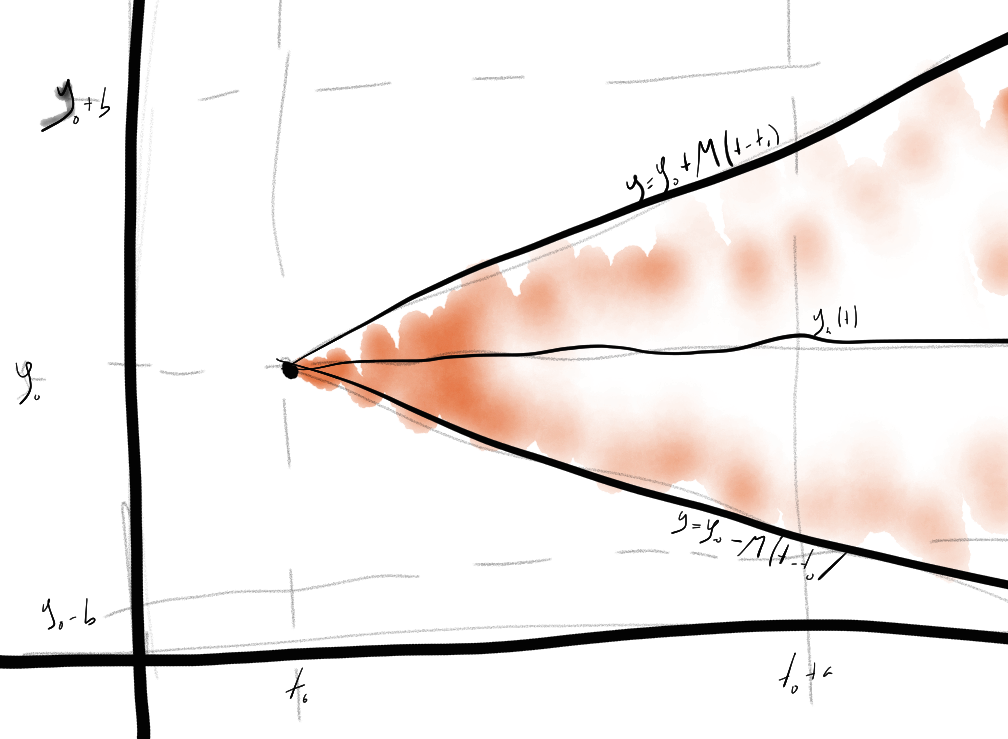
\includegraphics[width=0.8\textwidth]{./imagenes/2.PNG}
            \caption{\label{fig:pic}Grafica de dos soluciones aproximadas limite acotadas por un rectangulo $R$.}
        \end{figure}

		\begin{proof}
			\begin{align*}
				|y_n(t) - y_0| &= \left| \int_{t_0}^t f(s, y_{n-1}(s) ds) \right| \leq \int_{t_0}^t \left| f(s, y_{n-1}(s)) ds \right| \leq M \int_{t_0}^t ds \\
				|y_n(t) - y_0| &\leq M(t - t_0)
			\end{align*}
		\end{proof}

%-------------------------------------------------------------------------------
	\newpage
	\subsection{Constante de Lipschitz}

		\begin{definicion}
			Una función $f(x, y)$ definida en un dominio $D$ se dice que satisface la condición de Lipschitz con respecto a $y$, si para cada $x, y_1, y_2$ tales que $(x, y_1), (x, y_2) \in D$ se cumple que:

			\begin{equation}
				|f(x, y_1) - f(x, y_2)| \leq k |y_1 - y_2|
			\end{equation}
		\end{definicion}

		\begin{proof}
			Del teorema del valor medio obtenemos que:

			\begin{equation}
				|f(x, y_1) - f(x, y_2)| = \left| \frac{\partial f(x, \xi)}{\partial y} (y_2 - y_1) \right| \leq \max{\frac{\partial f(x, \xi)}{\partial y} |y_2 - y_1|}
			\end{equation}

			para un $\xi \in D$.
		\end{proof}

		\begin{teorema}
			Sea $x_0, y_0 \in \mathbb{R}$, con una función $f(x, y)$ continua y que satisface la condición de Lipschitz con una constante de Lipschitz $k$.
			Sean dos soluciones aproximadas $y_1, y_2$ de la ecuación diferencial $y' = f(x, y)$, definidas para $|x - x_0| \leq h$ con errores $\epsilon_1$ y $\epsilon_2$ respectivamente.
			Definimos $P(x) = y_1(x) - y_2(x)$, $\epsilon = \epsilon_1 + \epsilon_2$, entonces:

			\begin{equation}
				\left| P(x) \right| \leq e^{k|x - x_0|} \left| P(x) \right| + \frac{\epsilon}{k} \left[ e^{k(x - x_0)} - 1 \right]
			\end{equation}
		\end{teorema}

		\begin{proof}
			La desigualdad $|x - x_0| \leq h$ define el intervalo $[x_0 - h, x_0 + h]$, aunque usaremos $[x_0, x_0 + h]$ sin que por esto se pierda generalidad en la verificación.

			Las soluciones cumplen:

			\begin{align*}
				\left| \frac{d y_1}{dx} - f(x, y_1) \right| &\leq \epsilon_1 \\
				\left| \frac{d y_2}{dx} - f(x, y_2) \right| &\leq \epsilon_2
			\end{align*}

			Ahora notemos que:

			\begin{align*}
				\left| P'(x) \right| &= \left| \frac{d y_1}{dx} - \frac{d y_2}{dx} \right| \\
				&= \left| \frac{d y_1}{dx} - \frac{d y_2}{dx} + f(x, y_1) - f(x, y_1) + f(x, y_2) - f(x, y_2) \right| \\
				&= \left| \underbrace{\frac{d y_1}{dx} - f(x, y_1)}_{\leq \epsilon_1} - \underbrace{\frac{d y_2}{dx} + f(x, y_2)}_{\leq \epsilon_2} + \underbrace{f(x, y_1) - f(x, y_2)}_{\leq k|y_1 - y_2|} \right| \\
				\left| P'(x) \right| &\leq \epsilon_1 + \epsilon_2 + k|y_1 - y_2|
			\end{align*}

			lo cual implica que:

			\begin{equation*}
				\left| P'(x) \right| \leq k \left| P(x) \right| + \epsilon
			\end{equation*}
		\end{proof}
